\documentclass{standalone}
\usepackage[svgnames]{xcolor} % appeler le package avant les autres !
\usepackage{pstricks,pst-plot,pstricks-add,pst-3dplot}
\usepackage{pst-func}
\usepackage{pst-eucl,pst-calculate}
\usepackage{amsmath}
\usepackage{bm}
\usepackage{graphicx}
\definecolor{cgrille}{gray}{0.3}
\definecolor{foncred}{RGB}{213,35,35}
\definecolor{foncblue}{RGB}{65,113,162}
\definecolor{foncgreen}{RGB}{100,162,65}
\definecolor{foncpurple}{RGB}{121,78,200}
\definecolor{foncyellow}{RGB}{187,182,56}



\begin{document}
\psset{showpoints=false, % affichage des points
	   dotstyle=*, % style de point
	   dotsize=3pt, % taille de point
	   linewidth=1.5pt, % épaisseur des traits
	   subgriddiv=1, % grille divisée aux unités
	   griddots=8, % nombre de points sur le cˆot´e du carreau
	   subgriddots=10,
	   gridlabels=0pt, % taille des étiquettes
	   gridwidth=0.6pt, % épaisseur du trait de quadrillage
	   xunit=0.75cm, % facteur d'unité en abscisse
	   yunit=0.75cm, % facteur d'unité en ordonnée
	   runit=0.75cm, % facteur d'unité en radial
	   gridcolor=darkgray,
	   subgridcolor=darkgray,
	   algebraic=true} % couleur de la grille	            % psset est placé à l'intérieur de "figure" pour que les paramètres restent locaux.
\begin{pspicture}(-0.5,0)(11,5)
%\psgrid(0,0)(0,0)(11,7)
%\psaxes[labels=all,ticksize=3pt,ticks=all,labels=all,labelFontSize=\scriptstyle]{->}(0,0)(-5,-3)(5,10)


%%%%%%%%%%%%%%%%%%%%%%%%%%%%%%%%%%%%%%%%%%%%%%%%%%%%%%%%%%%%%%%%%%%%%%%%%%%%%%%%%%%%%%%%%%%
%%%%%%%%%%%%%%%%%%%%%%%%%%%%%%%%%%%%%%%%%%%%%%%%%%%%%%%%%%%%%%%%%%%%%%%%%%%%%%%%%%%%%%%%%%%

%\uput{1mm}[0]{0}(0.5,2.5){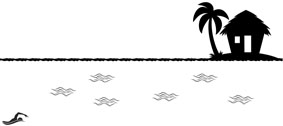
\includegraphics[scale=0.8]{Nageur.jpg}}
\rput(5.5,2.5){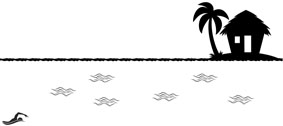
\includegraphics[scale=0.8]{Nageur.jpg}}

\psline[linecolor=darkgray,linestyle=dashed, dash=6pt 3pt,linewidth=2pt,arrows=<->](0.5,0.4)(0.5,2.6)
\psline[linecolor=darkgray,linestyle=dashed, dash=6pt 3pt,linewidth=2pt,arrows=<->](0.5,2.2)(9.5,2.2)
\psline[linecolor=darkgray,linewidth=1.2pt,arrows=-](0.5,0.3)(3,2.65)

\pstGeonode[PosAngle=90, PointNameSep=3mm,PointName=P, PointSymbol=*, dotscale=1.7](3,2.65){P}
%\psdot[dotscale=1.7](3,2.63)
\pstGeonode[PosAngle=90, PointNameSep=3mm,PointName=A, PointSymbol=*, dotscale=1.7](0.5,2.65){A}

\uput{2mm}[0]{90}(-0.4,1.4){$0,57\;km$}
\uput{1mm}[0]{0}(5,1.7){$2,8\;km$}



%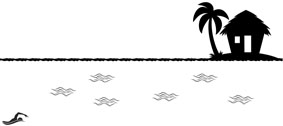
\includegraphics[scale=0.8]{Nageur.jpg}




\end{pspicture}
\end{document}